%-----------------------------------------------------------------------------%
\chapter{\babTiga}
%-----------------------------------------------------------------------------%

%-----------------------------------------------------------------------------%
\section{Alur Penelitian}
%-----------------------------------------------------------------------------%
Dalam suatu penelitian, terdapat urutan tahapan yang perlu dilakukan. Alur penelitian ini mengandung seluruh langkah yang harus ditempuh, mulai dari fase perancangan hingga tahap akhir penelitian.
 \begin{figure}
	\begin{center}
		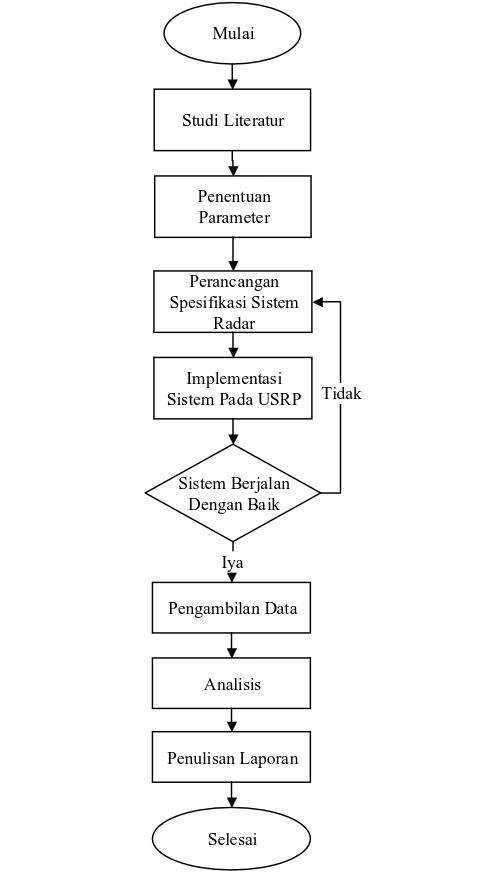
\includegraphics[scale=0.5]{pics/bab3/flowchart2.png} 
		\label{img:gambar 1}
		\caption[\textit{Flowchart} Penelitian]{\textit{Flowchart} Penelitian}
	\end{center}
\end{figure}
Pada alur penelitian yang telah dirancang, terdapat 6 tahap yang perlu dilakukan setelah penelitian dimulai dan sebelum penelitian diakhiri. Tiap tahapan yang telah dirancang harus dilaksanakan sebaik mungkin agar hasil yang diharapkan dapat tercapai.

\section{Studi Literatur}
Pada tahap ini, dilakukan studi literatur terhadap masalah yang diangkat serta solusi yang diajukan pada proposal ini. Studi literatur meliputi kajian artikel terdahulu hingga kajian terhadap perangkat lunak yang digunakan serta metode yang dilakukan dalam penyelesaian masalah.
	
\section{Penentuan Parameter}


\section{Perancangan Spesifikasi Sistem}
Pada tahap ini, dilakukan perancangan tentang penelitian yang diangkat, dalam konteks ini adalah radar. Sehingga perlu dilakukannya penentuan spesifikasi radar berdasarkan perangkat keras yang digunakan. Penelitian ini menggunakan alat USRP berseri B210.  Spesifikasi dari alat ini akan dijelaskan pada tabel berikut.

\begin{longtable}{|c|c|c|c|}
	\hline
	No. & Keterangan & Nilai & Satuan \\
	\hline
	1. & \textit{RF Coverage} & 70 - 6 & MHz - GHz \\
	\hline
	2. & \textit{Analog to Digital Converter Sample Rate} (maksimum) & 61.44 & MS/s \\
	\hline
	3. & \textit{Analog to Digital Resolution}  & 12 & bits	\\
	\hline
	4. &\textit{Analog to Digital Wideband SFDR} & 78 & dBc \\
	\hline
	5. & \textit{Digital to Analog Converter Sample Rate} (maksimum) & 61.44 & MS/s \\
	\hline
	6. & \textit{Digital to Analog Resolution}  & 12 & bits	\\
	\hline
	7. & \textit{Host Sample Rate} (16b) & 61.44 & MS/s \\
	\hline
	8. & \textit{Frequency Accuracy} & $\pm 2.0$ & ppm \\
	\hline
	9. &  \textit{W/ GPS Unlocked TCXO Reference} & $\pm 75$ & ppb \\
	\hline
	10. & \textit{W/ GPS Locked TCXO Reference} & $<$ 1 & ppb \\ 
	\hline
\end{longtable}

Dengan spesifikasi tersebut, maka USRP B210 memiliki kemampuan \textit{instantneous bandwidth} hingga 56 MHz pada transmisi 1 X 1 dan 30.72 MHz pada transmisi 2 X 2.

\section{Implementasi Sistem}
Tahap implementasi dilakukan dengan menerapkan hasil dari tahap perancangan pada alat USRP yang digunakan. 

\section{Evaluasi Sistem}
Tahap ini berguna untuk menguji sistem yang telah   perancangan.
	
\section{Pengambilan Data}
Pada tahap ini, pengambilan data dengan radar yang sudah didesain dan diimplementasikan pada USRP dilakukan.
%\todo{Skema konfigurasi percobaan dan pengujian jarak}

\section{Penentuan Spesifikasi Radar}
Dari studi literatur yang telah dilakukan, maka ditemukan parameter yang perlu di perhitungkan dalam melakukan perancangan radar FMCW, yaitu.
\begin{center}
\begin{longtable}{| c | c | c |}
	\caption[Spesifikasi Radar]{Spesifikasi Radar yang Diharapkan}
	\label{tab:spekRadar}\\
	\hline
	No. & Spesifikasi & Keterangan\\
	\hline
	1. & USRP & B210\\
	2. & \textit{Center Frequency} & 3 GHz \\
	3. & \textit{Bandwidth} & 56 MHz \\
	4. & Jarak & A m \\
	5. & Resolusi Jarak & A m \\
	6.& Kecepatan & A $m/s$ \\
	7. & Resolusi Kecepatan & A $m/s$\\
	\hline
\end{longtable}
\end{center}

Tabel \ref{tab:spekRadar} menjelaskan tentang spesifikasi radar yang dirancang dalam melaksanakan penelitian ini. Dengan spesifikasi tersebut diharapkan dapat mencapai tujuan yang sudah diangkat dan berhasil memberikan manfaat.